\documentclass[runningheads]{llncs}

\bibliographystyle{splncs04}% the mandatory bibstyle

\usepackage{txfonts}
\usepackage[T1]{fontenc}
% T1 fonts will be used to generate the final print and online PDFs,
% so please use T1 fonts in your manuscript whenever possible.
% Other font encondings may result in incorrect characters.
%
\usepackage{graphicx}
% Used for displaying a sample figure. If possible, figure files should
% be included in EPS format.
%
\usepackage{subcaption} %% For complex figures with subfigures/subcaptions
                        %% http://ctan.org/pkg/subcaption
\usepackage{uri}
\usepackage{mathpartir}
\usepackage{semantic}
\usepackage{cases}
\usepackage{hyperref}
% If you use the hyperref package, please uncomment the following two lines
% to display URLs in blue roman font according to Springer's eBook style:
\usepackage{color}
\renewcommand\UrlFont{\color{blue}\rmfamily}
\usepackage{stmaryrd}
\usepackage{listings}
\usepackage{amssymb}
\usepackage{iris-llncs}
%\usepackage{lstlangcoq}
\usepackage[edges]{forest}
\renewcommand{\lstlistingname}{Figure}

\clubpenalty = 10000
\widowpenalty = 10000
\displaywidowpenalty = 10000

\lstset{language=C,basicstyle=\ttfamily,mathescape=true,columns=fullflexible}

\newcommand{\TODO}[1]{\textbf{\textcolor{red}{[ TODO: #1]}}}
%\newcommand{\boxdotright}{\!\mathrel\boxdot\joinrel\rightarrow\!}
\newcommand{\islock}{\boxdotright}
\newcommand{\lockvar}{\islock^{v}}
\newcommand{\isaex}{\!\mathrel\odot\joinrel\rightarrow\!}
\newcommand{\xisaex}[1]{\!\mathrel\odot\joinrel\xrightarrow{#1}\!}
%% \newcommand{\ifthenelse}[3]{\text{if }#1\text{ then }#2\text{ else }#3}
\newcommand{\emp}{\mathsf{emp}}

\newcommand\dboxed[1]{\dbox{\ensuremath{#1}}}
\newcommand{\master}[2]{\ensuremath{\mathrm{Master}_{#1}(#2)}}
\newcommand{\snap}[1]{\ensuremath{\mathrm{Snapshot}(#1)}}
\newcommand{\ghost}[2]{\ensuremath{\dboxed{#1}^{#2}}}
\newcommand{\us}{$\mu$s}
\newcommand{\gnamety}{\ensuremath{\mathsf{gname}}}
\newcommand{\treerep}{\ensuremath{\mathsf{bst\_abs}}}
\newcommand{\nodeboxrep}{\ensuremath{\mathsf{bst\_ref}}}

\newcommand{\myhalf}[2]{\ensuremath{\mathsf{my\_half}_{#1}(#2)}}
\newcommand{\publichalf}[1]{\ensuremath{\mathsf{public\_half}(#1)}}

\newcommand{\ignore}[1]{}

\hyphenation{Comp-Cert}

\usepackage[utf8]{inputenc}

\begin{document}

\title{Proving Atomic Specifications for Data Structures with Fine-Grained Locking\thanks{Supported by the NSF (details).}}
%
%\titlerunning{Abbreviated paper title}
% If the paper title is too long for the running head, you can set
% an abbreviated paper title here
%
\author{Roshan Sharma\inst{1} \and
Shengyi Wang\inst{2}\orcidID{?} \and
Alexander Oey\inst{3} \and
Anastasiia Evdokimova\inst{4} \and
Lennart Beringer\inst{2}\orcidID{?} \and
William Mansky\inst{4}\orcidID{0000-0002-5351-895X}}

\authorrunning{R. Sharma et al.}

\institute{Amazon, USA \and Princeton University, USA \and Cisco, USA \and University of Illinois Chicago, USA} %do we need a note about prior affiliations?

%\ccsdesc[100]{\textcolor{red}{Replace ccsdesc macro with valid one}} https://dl.acm.org/ccs/ccs_flat.cfm 

%\nolinenumbers %uncomment to disable line numbering

\maketitle

\begin{abstract}
Logical atomicity has been widely accepted as a specification format for data structures in concurrent separation logic. While both lock-free and lock-based data structures have been verified against logically atomic specifications, most of the latter start with atomic specifications for the locks as well. In this paper, we compare this approach with one based on older lock-invariant-based specifications for locks. We show that we can still prove logically atomic specifications for data structures with fine-grained locking using these older specs, but the proofs are significantly more complicated than those that use atomic lock specifications. Our proof technique is implemented in the Verified Software Toolchain, which relies on older lock specifications for its soundness proof, and applied to C implementations of lock-based concurrent data structures.

\keywords{concurrent separation logic, fine-grained locking, logical atomicity, Verified Software Toolchain}
\end{abstract}

% Contributions:
% verified C implementation of BST -- the first?
% technique for hand-over-hand locking with share accounting -- slight modification of Gotsman's for logics without held predicates that remember the invariant; amounts to converting Locked_I into another share of the lock assertion
% technique for connecting locks with abstract state/atomicity
% VST-style decomposition of proofs into C-to-local-abstract and local-to-global-abstract
% lock-free implementation?

\section{Introduction}
The binary search tree (BST) is a common implementation of an ordered
map, a widely used data structure. The concurrent version of the
ordered map forms the bedrock of many parallel programs. We formally
verified the functional correctness of two versions of fine-grained
concurrent binary search trees (CBST) written in C. One adopts the
hand-over-hand locking technique \cite{bayer1977}, the other is lock
free by using atomic primitives such as compare and swap (CAS). Both
CBST implementations support insert, lookup, and delete operations; %or do we have lock-free without delete?
they also share the ``same'' specifications to some extent in our
verification. All the proof is machine-checked in Coq. %Say something about existing proofs of fine-grained data structures and how we compare.

Our specifications use the logical atomicity introduced in the TaDA
logic \cite{tada}, in the form of \emph{atomic Hoare
triples}. Intuitively, an atomic Hoare triple $ \langle
P \rangle\,\mathbb{C}\, \langle Q \rangle$ means the program
$\mathbb{C}$ ``atomically updates'' from $P$ to $Q$. The program may
actually take multiple steps, but every step before the atomic update
(linearization point) must preserve the assertion $P$. Meanwhile, the
concurrent environment may also update the state before the
linearization point, as long as the states satisfies $P$. The
assertion $Q$ must become true at the linearization point, then the
environment can do whatever it likes. There is no guarantee that $Q$
is still preserved when $\mathbb{C}$ returns. For example, the
specification of our \texttt{insert} operation may be explained as
follows: during the execution of \texttt{insert}, there is
always \emph{some} BST, and at some point the \texttt{insert} will
take a BST $t$, insert a value with a certain key, and then eventually
returns (meanwhile other threads may have further modified the
inserted tree)\footnote{Maybe say what a reasonable $Q$ is and why such a spec is still useful, specifically w.r.t. the situation where one of the other threads' action following the linearization point removes the element just inserted.}.

We employ the Verified Software Toolchain (VST) \cite{plfcc} to verify
the correctness of CBST. Although the concurrent separation logic
(CSL) has been formalized in VST rooted on the work of Hobor et
al.\ \cite{oraclesematic}, we extend it with two descendants of CSL so
as to accomplish the verification. One is the logical atomicity
mentioned above; the other is the higher-order ghost state in the
style of Iris \cite{higherorderghoststate}. The ghost states are used
to contruct both the global invariants and the local state in our
proofs. They will be further discussed in \S\ref{correctness}.

We highlight a few innovative aspects of our verification of CBST:
\begin{description}
\item [Range ghost] We abstract the BST via a pair of values
called \emph{range} which represents the lower-bound and upper-bound
of keys on each node to reason about the BST in the current
settings. We prove that range with the merging operation forms a
partial commutative monoid (PCM) so that it can be encoded in ghost
states.

\item [\textsf{sync\_inv} pattern] It is a particular approach
combining locks with general invariants to solve the dilemma caused by
the fine-grained locking mechanism: we do not have a lock to control
the access of the entire BST nor can we access the state of the BST
via atomic operations.
\end{description}

%% Do we have contributions, and are they sufficient? Range ghost is adapted from flow interfaces. Sync_inv pattern isn't totally ours, though it might be instructive w.r.t. combining traditional and Iris-style CSLs, and it might be worth explaining in more detail. We're working on "actual" code, but missing a few pieces to make our proofs foundational. (but maybe it's worth highlighting the extra work we do to work on actual code) We could promote this as the first working example of Iris+VST. We don't yet have any demonstrations on larger or interesting data structures, and this alone was quite a bit of work. The delete logic is rather interesting. Nothing to say about flow interfaces yet, but maybe soon.


Our specific contributions are:
\begin{itemize}
\item To the best of our knowledge, this is the first mechanized
verification of an concurrent search-based data structure written in a
real programming language. %should probably clarify what we mean by "real"

\item We illustrate how to incorporate the CSL in VST, the higher-order
ghost state in the style of Iris, and the logical atomicity from the
TaDA logic together to verify the CBST.
\end{itemize}

We introduce the background about the verification of concurrent C
programs in \S\ref{background}, including the tool-chain VST and Iris,
the concept of ghost states, global invariants, and atomic
specifications. The thread-safety proofs of operations on CBST are
first explained in \S\ref{safety}, where we show the \emph{recursive}
lock pattern for hand-over-hand locking mechanism. The functional
correctness proofs are presented in \S\ref{correctness}. We detail the
use of the \textsf{sync\_inv} pattern, the combination of recursive
lock invariants and ghost states together in the atomic
specifications, and the proof skeleton of each operation on CBST. The
related work is discussed in \S\ref{related}. We end with the
conclusion of our work in \S\ref{conclusion}.



\section{Background}
\label{background}

\subsection{Two Styles of Lock Specification}
Soon after the introduction of concurrent separation logic~\cite{csl}, both Gotsman et al.~\cite{gotsman} and Hobor et al.~\cite{oraclesematic} extended it with support for C-style storable locks, where a lock is a special memory location designated as coordinating access to some other resource. Their lock specifications were essentially equivalent, and of the form:
$$\{ \ell \islock R \}\ \texttt{acquire}(\ell)\ \{ R * \ell \islock R \} \qquad \{ R * \ell \islock R \}\ \texttt{release}(\ell)\ \{ \ell \islock R \}$$
Each lock $\ell$ is associated with a ``lock invariant'' $R$, an arbitrary separation logic predicate representing the protected resource, which is gained by a thread that acquires the lock and must be restored when the lock is released. At the time, there was no formal treatment of atomic operations in CSL, so actual lock implementations were beyond the scope of verification: these specs were taken as axioms, or proved through direct appeal to data-race-free guarantees of specific memory models.

Later, the TaDA logic~\cite{tada} presented an alternative set of lock specifications, based on the newly introduced notion of logical atomicity:
$$\langle b.\ (\mathsf{L}(\ell) \land \neg b) \vee (\mathsf{U}(\ell) \land b) \rangle\ \texttt{acquire}(\ell)\ \langle \mathsf{L}(\ell) \land b \rangle \qquad \langle \mathsf{L}(\ell) \rangle\ \texttt{release}(\ell)\ \langle \mathsf{U}(\ell) \rangle$$
An \texttt{acquire} operation may access the lock repeatedly, finding it in either the locked ($\mathsf{L}$) or unlocked ($\mathsf{U}$) state; if it sees the unlocked state ($b$ holds), then it can atomically move to a locked state and return. A release simply moves atomically from the locked state to the unlocked state. These operations make no mention of a protected resource, but because they are atomic, they can interact with any global invariant (``shared region'' in TaDA's terminology): in particular, in combination with the invariant $(U(\ell) * R) \vee L(\ell)$, they can be used to derive the lock-invariant-based specs. It is also worth noting that these lock specifications are not axioms: they are proved for a simple spinlock implementation that uses atomic operations (e.g. compare-and-swap), which are the actual primitive operations in TaDA and the logics that follow it.

\subsection{VST and Iris}

The Verified Software Toolchain (VST)~\cite{plfcc} is a Coq-based system for proving separation logic specifications of C programs. It is proved sound against not only the C semantics of the CompCert compiler, but also the compiler correctness theorem~\cite{cpm}, so that verified programs are guaranteed to behave correctly when compiled and run. VST directly implements the concurrent separation logic of Hobor et al.~\cite{oracle-sematics}, and the invariant-style lock specifications are incorporated into its soundness proof at a fundamental level.

Iris~\cite{iris} is a Coq-based separation logic framework that synthesizes ideas from a range of CSLs with the idea that ``ghost state is all you need''. Iris begins with a small core logic including arbitrary higher-order ghost state, and derives features including invariants and logical atomicity from particular instances of ghost state. Iris is designed as a language- and logic-independent framework, and recent versions of VST take advantage of this, incorporating Iris-style ghost state in the foundational model and directly using Iris tactics to reason about invariants and atomicity. All proofs described in this paper have been formalized in this VST+Iris setting.
%What else do we need to say?

\ignore{\subsection{Ghost State and Global Invariants}
We can prove memory safety and race freedom properties of shared-memory concurrent programs, by tracking the transfer of ownership of shared locations between threads that would happen if we ran the program. But, this idea is insufficient to prove that concurrently running threads are successful to accomplish some task, which is also called functional correctness. For instance, we can prove the memory safety properties of the increment example in  \ref{figure1} through the transfer of ownership of shared variable $x$ between threads. But, we can not guarantee that the value of $x$ will be $2$ after all threads complete their execution, which is demonstrated in \ref{figure1} using separation logic assertion.   
\begin{figure}[htb]
\centering
$\texttt{x = 0;}$\\
$\mathit{I_{\pi}(x \mapsto v \land v \geq 0)}\qquad\pi = \pi_1\ .\ \pi_2$\\
$\begin{array}{l || l}
\mathit{I_{\pi_1}(x \mapsto v \land v \geq 0)} & \mathit{I_{\pi_2}(x \mapsto v \land v \geq 0)}\\
\texttt{acquire(l);} & \texttt{acquire(l);}\\
\mathit{x \mapsto v \land I_{\pi_1}(x \mapsto v \land v \geq 0)} & \mathit{x \mapsto v \land I_{\pi_2}(x \mapsto v \land v \geq 0)}\\
\texttt{x++;} & \texttt{x++;}\\
\mathit{x \mapsto v+1 \land I_{\pi_1}(x \mapsto v \land v \geq 0)} & \mathit{x \mapsto v+1 \land I_{\pi_2}(x \mapsto v \land v \geq 0)}\\
\texttt{release(l);} & \texttt{release(l);}\\
\mathit{I_{\pi_1}(x \mapsto v \land v \geq 0)} & \mathit{I_{\pi_2}(x \mapsto v \land v \geq 0)}\\
\end{array}$\\
$\mathit{I_{\pi}(x \mapsto v \land v \geq 0)}$
\caption{The increment example annotated with separation logic assertion}
\label{figure1}
\end{figure}
We must preserve the connection between the value of shared resources and the work performed by each thread. A common approach to achieve this is to use \emph{ghost variables}, an auxiliary state introduced later in the proof to track the local information about each thread. They do not appear in the original program. Program in \ref{figure1} can be verified by creating ghost state, which tracks the latest action performed by a thread, for each thread with initial value of $0$, and update with $1$ after each thread increment the value of \texttt{x}. In VST, we can create \emph{ghost state} for any Coq type in the form of an arbitrary \emph{partial commutative monoid} (PCM), a set with a partially defined binary operation that is as associative as it can, commutative, and has a unit, as long as we can describe what happens when two elements of that type are joined together. VST provides $\mathsf {ghost\_var}$ assertion to create a simple ghost state: $\mathsf{ghost\_var}\ \mathit{sh}\ a\ g$ asserts that $g$ is a \emph{ghost name} ($\gnamety$ in Coq) associated with the value $a$, which may be of any type. We will see different kind of ghost states used to verify binary search tree in the following sections.

The main idea behind the logic from Iris \cite{higherorderghoststate}, a mechnized higher-order concurrent separation logic framework, is the construction of \emph{global invariant} as \emph{ghost state}. \emph{Global Invariant} is an invariant on the global (ghost and physical) state of program. We can open any invariant but must close it again before taking any steps of execution unless those execution are atomic. Thread can use the contents of \emph{global invariant} during atomic operation if it can guarantee that no one will ever see an intermediate state in which invariant does not hold. The rules from Jung et al.\cite{higherorderghoststate} for creating and opening invariants are:

\begin{mathpar}
\inference[\textsf{inv\_alloc}]{}{\triangleright P \vdash \pvs[E] \mathsf{EX}\ i : \mathsf{iname}, \knowInv{i}{P}}

\inference[\textsf{inv\_open}]{i \in E}{\knowInv{i}{P} \vdash \pvs[E][E \setminus i] \triangleright P * (\triangleright P \wand \pvs[E \setminus i][E] \mathsf{emp})}
\end{mathpar}

where invariants are provided in the form of assertion $\knowInv{i}{P}$, and states that $P$ is maintained as an invariant on the global state with name $i$. The operator%%  $\pvs[][]$
is called ``fancy update" operator,that allows to allocate, open, and close the invariants and the later $\triangleright$ operator is used for impredicativity (i.e. $\knowInv{i}{..\knowInv{i}{P}..}$).}

\ignore{\subsection{Atomic Specifications}
\label{atomic}

For many concurrent data structures, the ideal correctness condition is that the data structure behaves the same as a sequential implementation, even when accessed simultaneously by multiple threads. This intuitive condition can be formalized as linearizability (operations appear to take effect in some total order) or atomicity (client threads never observe intermediate states of operations). In separation logic, atomicity can be expressed in the form of \emph{atomic triples}~\cite{tada}, written in the form $\forall a.\ \langle P_l\ |\ P_p(a)\rangle\ c\ \langle Q_l\ |\ Q_p(a)\rangle$, where $P_l$ and $Q_l$ are \emph{private} pre- and postconditions similar to an ordinary Hoare triple, and $P_p$ and $Q_p$ are \emph{public} pre- and postconditions, parameterized by an abstract value $a$ of the shared data structure. Intuitively, $P_l$ and $Q_l$ must be true before and after the call, while $P_p$ must be true for some value of $a$ at every point from the beginning of $c$ until some designated linearization point, at which point $Q_p$ becomes true atomically for the same value $a$. For instance, the specification $$\forall s.\ \langle \mathsf{is\_stack}\ p\ |\ \mathsf{stack}\ s\rangle\ \texttt{push}(v)\ \langle \mathsf{is\_stack}\ p\ |\ \mathsf{stack}\ (v :: s)\rangle$$ expresses the fact that the \texttt{push} operation of a concurrent stack correctly implements the behavior of a sequential push, atomically transitioning from some stack $s$ to $v :: s$ at some point during its execution. %maybe something about linking ghost state, which parts are real vs. ghost, accessing invariants around atomic triple
%Maybe say what a reasonable $Q$ is and why such a spec is still useful, specifically w.r.t. the situation where one of the other threads' action following the linearization point removes the element just inserted.

VST has encoded an atomic Hoare triple, and provide the way that matches the notation VST uses for normal specifications. Such specification is called \emph{atomic specification}, and can be formalized in Coq as shown in  \ref{atomic-spec}.  This is how we write pre- and postcondition in VST. 
\begin{figure}[htb]
\centering
\begin{verbatim}
Program Definition insert_spec :=
DECLARE _insert
ATOMIC TYPE W OBJ a INVS Ei Eo
WITH ...
PRE [ ... ]
  PROP (...)
  LOCAL (...)
  SEP (P_l) | (P_p)
POST [ ... ]
  PROP ()
  LOCAL ()
  SEP (Q_l) | (Q_p)
\end{verbatim}
\caption{Atomic Specification in VST}
\label{atomic-spec}
\end{figure}
\texttt{W} is the \textsf{TypeTree} representing the type of arguments passed with \texttt{WITH} clause; \texttt{a} is the abstract state for the triple; \texttt{Ei} and \texttt{Eo} are the sets of invariants names inside and outside the triple. The \texttt{PROP} clause describes things that that are true independent of program state, the \texttt{LOCAL} clause describes the values contained in C local variables, and the \texttt{SEP} clause represents the \emph{separating conjunction} (*) of \emph{spatial predicates}, predicates on some part of the memory. In VST, while proving that a function implements an atomic specification, the precondition will contains an $\mathsf{atomic\_shift}$ assertion with the public pre- and postcondition, and the masks inside it. This atomic shift can be accessed through following two rules:
$$\inference[\textsf{atomic\_commit}]{\forall a, R * P_p\ a \Rrightarrow \mathsf{EX}\ y,\ Q_p\ a\ y * R'\ y}{\textsf{atomic\_shift}(P_p, E_i, E_o, Q_p, Q) * R \Rrightarrow \mathsf{EX}\ y,\ Q\ y * R'\ y}$$
$$\inference[\textsf{atomic\_rollback}]{\forall a, R * P_p\ a \Rrightarrow P_p\ a * R'}{\textsf{atomic\_shift}(P_p, E_i, E_o, Q_p, Q) * R \Rrightarrow \textsf{atomic\_shift}(P_p, E_i, E_o, Q_p, Q) * R'}$$
During commit, we must provide resources $R$ which, in combination with the public precondition $P_p$, allow us to prove the public postcondition $Q_p$. Then, we gain access to an assertion $Q$ required by the postcondition of the function, and leftover resources $R'$. During rollback, we provide resources $R$ which, in combination with the public precondition, allow us to reestablish the public precondition; we then regain the atomic shift back in the proof, as well as leftover resources $R'$. The rollback is specially used to learn some relationship between pieces of information (e.g. ghost state) stored in the public precondition, while the commit is used to prove the public postcondition from the precondition, and obtain an assertion $Q$. To complete the proof of any function's specification, we must always perform commit to obtain $Q$; we can perform any number of rollbacks before that point, but after that point we lose the atomic shift and no access to the public precondition.}

\section{Locks and Atomicity}
Suppose we have a sequential implementation of a binary search tree. It has functions \texttt{insert}, \texttt{lookup}, and \texttt{delete}, proven to satisfy the following specifications:
\begin{mathpar}
\{\mathsf{BST}\ p\ t\}\ \texttt{insert}(p, k, v)\ \{\mathsf{BST}\ p\ (\mathsf{insert}\ t\ k\ v)\}

\{\mathsf{BST}\ p\ t\}\ \texttt{lookup}(p, k)\ \{v.\ \mathsf{BST}\ p\ t \land \mathsf{lookup}\ t\ k = v\}

\{\mathsf{BST}\ p\ t\}\ \texttt{delete}(p, k)\ \{\mathsf{BST}\ p\ (\mathsf{delete}\ t\ k)\}
\end{mathpar}
where $\mathsf{BST}\ p\ t$ asserts that some abstract binary search tree $t$ is represented in memory starting at location $p$. For instance, $t$ may be a recursively defined tree type in Coq, and $\mathsf{insert}$ may be a pure Coq function that adds a key-value pair to such a tree; $\mathsf{BST}$ could then be defined as a recursive predicate that represents each node of $t$ as an object in memory, with fields for key, value, and pointers to left and right children, and $p$ could be the location of the root node.

A thread-safe version of this data structure should satisfy atomic specifications that closely correspond to the sequential specs:
\begin{mathpar}
\forall t.\ \langle \nodeboxrep\ p\ |\ \treerep\ t\rangle\ \texttt{insert}(p, k, v)\ \langle \nodeboxrep\ p\ |\ \treerep\ (\mathrm{insert}\ t\ k\ v)\rangle

\forall t.\ \langle \nodeboxrep\ p\ |\ \treerep\ t\rangle\ \texttt{lookup}(p, k)\ \langle v.\ \nodeboxrep\ p\ |\ \treerep\ t \land \mathrm{lookup}\ t\ k = v\rangle

\forall t.\ \langle \nodeboxrep\ p\ |\ \treerep\ t\rangle\ \texttt{delete}(p, k)\ \langle \nodeboxrep\ p\ |\ \treerep\ (\mathrm{delete}\ t\ k)\rangle
\end{mathpar}
These specifications assert that each operation appears to execute atomically, accessing and updating the state of the data structure without exposing any intermediate states---for instance, a \texttt{lookup} should not find a partially inserted key with a value other than the one passed to its \texttt{insert} call. Our sequential implementation will almost certainly not satisfy these specifications, because its functions relied on being able to access any part of the data structure at any time: in separation logic terms, the $\mathsf{BST}$ assertion included full ownership of every location in the data structure.

\subsection{Atomicity with lock invariants}
The easiest way to synchronize a data structure is to add a lock that each operation acquires at the start and releases at the end. With the invariant-style lock specs, we can make $\mathsf{BST}\ p\ t$ the invariant of this lock: the lock then holds full ownership of the data structure, and provides it to whichever thread is currently executing an operation on the tree at $p$.
In this \emph{coarse-grained} locking implementation, any thread with partial ownership of the lock can acquire the lock, perform all the operations of the sequential insertion/lookup/deletion, and then release the lock. Naively, we might choose as our lock invariant $\exists t.\ \mathsf{BST}\ p\ t$, asserting that we gain full ownership of the tree in some state $t$ every time we acquire the lock---but this is not enough to tell us that we have changed the lock's state by the end of the operation, since we merely restore the invariant that there is \emph{some} tree $t$ at $p$. This is where ghost state and atomic triples come in: we can define a piece of ghost state $\mathsf{ghost\_bst}\ t$ that is divided between the lock invariant and the public pre- and postconditions of the functions, connecting the tree in memory to the public abstract state of the data structure. For instance, we might choose a lock invariant $R_{\mathit{cg}} \triangleq \exists t.\ \mathsf{BST}\ p\ t * \mathsf{ghost\_bst}_{.5}\ t$, and then set $\nodeboxrep\ p \triangleq p \islock R_{\mathit{cg}}$ and $\treerep\ t \triangleq \mathsf{ghost\_bst}_{.5}\ t$. Then we can prove the atomic triples above, where at the linearization point we access $\mathsf{bst\_abs}$, combine the two halves of the ghost state and update them to reflect the new state of the concrete data structure, and then satisfy the atomic postcondition with one half of the ghost state and return the other half to the lock invariant. The atomic postcondition reflects the fact that the abstract state has been accessed or changed, while the lock invariant maintains the connection between the abstract state and the actual data structure in memory. This approach to making changes to a locked data structure visible via ghost state is due to Zhang and Jung's proofs of an atomic syncer in Iris~\cite{atomic-syncer}.%, a higher-order function that wraps any arbitrary functionality in a lock. They proved that if a target function $f$ has a spec of the form $\{R * P\}\ f\ \{R * Q\}$, where $R$ is e.g. the ownership assertion for a data structure, then the locked version $f'$ of $f$ has spec $\langle g. P * \mathsf{ghost}_{.5}\ g\rangle\ f'\ \langle Q * \mathsf{ghost}_{.5}\ g'\rangle$.

\label{atomicity}

In a \emph{fine-grained} implementation, there are multiple locks on different pieces of the data structure, so the ghost state of each lock invariant cannot be the abstract state of the entire data structure. Instead, the ghost state represents the abstract state of the locked section alone, and the abstract state of the data structure is derived from the composition of the states of the locked components. Each locked component $c$ has a piece of ghost state $\mathsf{ghost}\_c$ that is split between the lock invariant and the top-level abstract state. At the end of a critical section for $c$, we atomically access the top-level abstract state, combine the two halves of $\mathsf{ghost}\_c$, update $\mathsf{ghost}\_c$ to reflect any local changes, and then show either that the update to $c$ does not change the top-level state of the data structure, or that the update to $c$ changes the top-level state to one that satisfies the atomic postcondition for the function. For instance, when deleting a node from a binary search tree, we rotate nodes to reconstruct a valid tree; at the end of the critical section for each rotation, we show either that the values in the tree are unchanged (and the tree is still well-ordered), or that we have removed the node to be deleted. %elaborate on two-level structure

\ignore{The construction of the lock variants is simple. We begin with a \emph{part-reference} ghost state, a common construction for sharing information between an invariant and the threads that act on it, with elements $\publichalf{a}$ (the current state $a$) and $\myhalf{\pi}{p}$ (partial information about the current state, annotated with a share $\pi$). When the share $\pi$ is 1, we know that $p = a$. (do we want to define this ourselves, or reference it somewhere? note also that this is what Iris calls an authoritative algebra) A lock variant with an assertion $R(a)$ is then defined as %notation
$$\ell \lockvar_\pi R \triangleq \ell \islock \exists a.\ R(a) * \myhalf{\pi}{a}$$ %eliding ghost names here
The share $\pi$ may be set to 1 if the lock's information about $a$ is always fully up to date, or a smaller share if it can become outdated due to operations on other parts of the data structure. Since $a$ is existentially quantified, a thread that changes the value of $a$ forgets it after releasing the lock (as required in a lock invariant), but it must have synchronized with a $\publichalf{a}$ held elsewhere (usually in a global invariant) that will remember the change. Thus, the ghost state acts as a bridge between the component lock invariant and the global abstract state of the data structure. %smaller example before we get into BST?
}

\ignore{From the atomic rules of section~\ref{atomic}, we derive the following rules for accessing and modifying pieces of the global abstract state:
\begin{mathpar}
\inference[\textsf{sync\_commit}]{\forall a.\ R * P_p\ a \Rrightarrow \exists x_1.\ \mathsf{public\_half}(g, x_1) * \exists x_0',\,x_1'.\ (x_0, x_1) \leadsto (x_0', x_1')\ \land \\(\mathsf{my\_half}(g, \mathit{sh}, x_0') * \mathsf{public\_half}(g, x_1') \Rrightarrow \exists y.\ Q_p\ a\ y * R'\ y)}{\textsf{atomic\_shift}(P_p, E_i, E_o, Q_p, Q) * \textsf{my\_half}(g,sh,x_0) * R \Rrightarrow \mathsf{EX}\ y,\ Q\ y * R'\ y}

\inference[\textsf{sync\_rollback}]{\forall a.\ R * P_p\ a \Rrightarrow \exists x_1.\ \mathsf{public\_half}(g, x_1) * (\mathsf{public\_half}(g, x_1) \Rrightarrow P_p\ a * R')}{\begin{array}{c}\textsf{atomic\_shift}(P_p, E_i, E_o, Q_p, Q) * \textsf{my\_half}(g,sh,x_0) * R  \Rrightarrow \\\textsf{atomic\_shift}(P_p, E_i, E_o, Q_p, Q) * \textsf{my\_half}(g,sh,x_0) * R'\end{array}}
\end{mathpar}
A thread that holds $\myhalf{}{a}$ (i.e., is in the critical section of a lock with a lock variant) may interact with the abstract state $P_p$ held in an $\textsf{atomic\_shift}$, as long as the corresponding $\publichalf{}$ is part of the abstract state. It may either leave both halves as is and gain updated resources $R'$ (including, e.g., a snapshot of the current abstract state), or update both halves to a new state that satisfies the public postcondition $Q_p$, executing the linearization point and obtaining the final postcondition $Q$. Typically we will use one of these rules at the end of each critical section, to show that the changes made in the critical section either are invisible to other threads (\textsf{sync\_rollback}) or have fulfilled the linearization point (\textsf{sync\_commit}). We can also derive simpler rules for special cases, such as a version of \textsf{sync\_commit} for read-only operations that do not change the state of any component:

$$\inference[\textsf{sync\_commit\_same}]{\forall a.\ R * P_p\ a \Rrightarrow \exists x_1.\ \mathsf{public\_half}(g, x_1) * (\mathsf{my\_half}(g, \mathit{sh}, x_0) * \mathsf{public\_half}(g, x_1) \Rrightarrow \exists y.\ Q_p\ a\ y * R'\ y)}{\textsf{atomic\_shift}(P_p, E_i, E_o, Q_p, Q) * \textsf{my\_half}(g,sh,x_0) * R \Rrightarrow \mathsf{EX}\ y,\ Q\ y * R'\ y}$$
}

\subsection{Atomicity with atomic locks}
Proving atomic specifications for a data structure using atomic specifications for locks is more immediate. As an example, consider Patel et al.'s verification of a hand-over-hand locking pattern for search structures~\cite{templates}. %outline how this worked for them

In particular, in the fine-grained case, there is no need to create extra ghost state to abstract the state of each locked component, and then synthesize it into a top-level abstract state for the data structure. Instead, each lock acquire and release can atomically access the top-level abstract state, and directly make changes there. It is even possible for a thread to acquire a lock without owning a share of the lock assertion: the lock assertion can be extracted directly from the top-level state during the atomic \texttt{acquire} operation, and returned when \texttt{acquire} returns. This completely circumvents the recursive-lock reasoning needed for hand-over-hand locking with lock-invariant specs. %This comes later in the current version.

\section{A Verified Binary Search Tree with Hand-over-Hand Locking}
\label{hand-over-hand}

We demonstrate our approach by verifying a binary search tree (BST) with fine-grained locking in VST, using the above approach to prove atomic specifications for the BST operations while using invariant-style specs for our locks (as required by VST's soundness proof).
As described in section~\ref{atomic}, we want the operations of our concurrent BSTs to satisfy atomic triples relating them to sequential operations:
\begin{mathpar}
\forall t.\ \langle \nodeboxrep\ p\ |\ \treerep\ t\rangle\ \texttt{insert}(p, k, v)\ \langle \nodeboxrep\ p\ |\ \treerep\ (\mathrm{insert}\ t\ k\ v)\rangle

\forall t.\ \langle \nodeboxrep\ p\ |\ \treerep\ t\rangle\ \texttt{lookup}(p, k)\ \langle v.\ \nodeboxrep\ p\ |\ \treerep\ t \land \mathrm{lookup}\ t\ k = v\rangle

\forall t.\ \langle \nodeboxrep\ p\ |\ \treerep\ t\rangle\ \texttt{delete}(p, k)\ \langle \nodeboxrep\ p\ |\ \treerep\ (\mathrm{delete}\ t\ k)\rangle
\end{mathpar}
In our case, insert, lookup, and delete are simple Gallina functions on a functional tree data structure. The details of $\nodeboxrep$ and $\treerep$ may vary by implementation, but we expect that $\nodeboxrep$ contains at least a pointer to the data structure, and $\treerep$ contains some ghost state linking the concrete state of the data structure to the abstract tree $t$.

In the following sections, we describe the construction of these predicates, and the proofs of the operations, for BST implementations based on hand-over-hand locking and lock-free atomic operations.

%look at some of the Iris papers in CPP, etc. for how we should describe the proofs, e.g. section 4 of Formal Verification of a Concurrent Bounded Queue in a Weak Memory Model, Mevel and Jourdan, ICFP 2021

%%%%%%%%%%%%%%%%%%%%%

\ignore{In the previous section, we showed that how to prove concurrent data-structure is thread safe, but not functionally correct. To prove the correctness, our threads need to be able to record the information about the actions they have performed on the shared state, instead of sealing all knowledge of the shared data structure inside the lock invariant. We can accomplish this with ghost variables, a simple form of auxiliary state. Aside from the \emph{permission} on shared resources held by each thread that we used in the safety proofs, the verification of correctness properties also involves the \emph{ghost state}. In VST, any Coq type can be used as ghost state, as long as we can describe what happens when two elements of that type are joined together. We can use own predicate in VST to represent ghost state assertion as follows: $\mathsf{own}\ g\ a\ \mathit{pp}$, where $g$ is a \emph{ghost name}, $a$ is the value associated with $g$ which can be of any type, and $\mathit{pp}$ is a separation logic predicate.}


%Linearizability is one of the most popular strong correctness condition for the most of %concurrent data-structure, which implies that every operation appears to take place atomically, %in some order, consistent with the real-time ordering of those operations. 
%In order to record the action each thread performed as a linear history, we will define global %invariants using the ghost state, which are similar to lock invariants but are not associated %with any particular memory location. Instead, a global invariant is true before and after every %step of a program, acting as a publicly accessible resource. A program instruction can use the %contents of global invariant if it can guarantee that no one will ever see an intermediate state %in which the invariant does not hold. 

\ignore{\subsection{BST code}
\label{selflock}

\begin{figure}[htp]
\begin{lstlisting}[language = C, basicstyle=\small\ttfamily]
typedef struct tree {int key; void *value; struct tree_t *left, *right;} tree;
typedef struct tree_t {tree *t; lock_t *lock;} tree_t;
typedef struct tree_t **treebox;
\end{lstlisting}
\begin{subfigure}[t]{0.5\textwidth}
\begin{lstlisting}[language = C, basicstyle=\small\ttfamily, numbers=left]
void insert (treebox t, int x, void *value) {
  struct tree_t *tgt = *t;
  struct tree *p;
  void *l = tgt->lock;
  acquire(l);
  for(;;) {
    p = tgt->t;
    if (p==NULL) {
      tree_t *p1 = malloc(sizeof *tgt);
      tree_t *p2 = malloc(sizeof *tgt);
      p1->t = NULL;
      p2->t = NULL;
      lock_t *l1 = malloc(sizeof(lock_t));
      makelock(l1);
      p1->lock = l1;
      release2(l1);
      lock_t *l2 = malloc(sizeof(lock_t));
      makelock(l2);
      p2->lock = l2;
      release(l2);
      p = malloc(sizeof *p);
      tgt->t = p;
      p->key=x; p->value=value; p->left=p1; p->right=p2;
      release(l);
      return;
    } else {
      int y = p->key;
      if (x<y){
      	tgt = p->left;
        void *l_old = l;
        l = tgt->lock;
        acquire(l);
        release(l_old);
      } else if (y<x){
        tgt = p->right;
        void *l_old = l;
        l = tgt->lock;
        acquire(l);
        release(l_old);
      } else {
      	p->value=value;
        release(l);
      	return;
      }
    }
  }
} 
\end{lstlisting} 
\end{subfigure}\qquad
\begin{subfigure}[t]{0.4\textwidth}
 \begin{lstlisting}[language = C, basicstyle=\small\ttfamily]
void *lookup (treebox t, int x) {
  struct tree *p; void *v;
  struct tree_t *tgt;
  tgt = *t;
  void *l = tgt->lock;
  acquire(l);
  p = tgt->t;
  while (p != NULL) {
    int y = p->key;
    if (x<y){
      tgt = p->left;
      void *l_old = l;
      l = tgt->lock;
      acquire(l);
      p = tgt->t;
      release(l_old);
    } else if (y<x){
      tgt = p->right;
      void *l_old = l;
      l = tgt->lock;
      acquire(l);
      p = tgt->t;
      release2(l_old);
    } else {
      v = p->value;
      release(l);
      return v;
    }
  }
  release(l);
  return NULL;
}
\end{lstlisting}
\end{subfigure}
\caption{BST with hand-over-hand locking}
\label{bst-conc}
\end{figure}
}

\subsection{Hand-over-Hand Locking}
\label{selflock}

Hand-over-hand locking (also called lock coupling) is a fine-grained locking pattern for traversing a data structure in which we acquire the lock for the next node before releasing the lock for the current node, thus guaranteeing that the link between the two nodes is not removed or rearranged while we traverse it. Hand-over-hand locking is a classic example of a pattern that requires reference to lock invariants inside other lock invariants, dating back to the earliest papers on ``predicates in the heap'' in CSL~\cite{gotsman}. The trick is to assign each node in the data structure a lock invariant that includes the lock assertion for its child nodes; for a linked list, for instance, we might write $R(n) \triangleq n \mapsto (d, n', \ell') * \ell' \islock R(n')$, where $n'$ is the child of $n$ and $\ell'$ is $n'$'s lock. By acquiring $n$'s lock, we learn the lock assertion for $n'$, and can acquire its lock as needed before releasing $n$.

This invariant becomes slightly more complicated when we consider \emph{ownership} of locks, as is required if we want to eventually free the lock and return its resources. In this case the lock assertion carries a share $\pi$, where the full share $\pi = 1$ is required to free the lock, while any share is sufficient to acquire or release it. We can amend our lock invariant to $R(n) \triangleq n \mapsto (d, n', \ell') * \ell' \islock_\pi R(n')$ for some suitable share $\pi$, but then, what happens to the share of $n_1$'s lock when we release the lock on $n$? Starting from a state in which we hold $n$'s lock $\ell$, this gives us:
$$\begin{array}{l}
\{ \ell \islock_\pi R(n) * n \mapsto (d, n', \ell') * \ell' \islock_\pi R(n') \}\\
\texttt{acquire}(\ell');\\
\{ \ell \islock_\pi R(n) * n \mapsto (d, n', \ell') * \ell' \islock_\pi R(n') * n' \mapsto (d, n'', \ell'') * \ell'' \islock_\pi R(n'') \}\\
\texttt{release}(\ell);\\
\{ \ell \islock_\pi R(n) * n' \mapsto (d, n'', \ell'') * \ell'' \islock_\pi R(n'') \}
\end{array}$$
In order to re-establish $\ell$'s lock invariant $R(n)$, we must give up our knowledge of $n'$'s lock $\ell'$. This leaves us with two problems: we have no lock assertion for $\ell'$, so we will be unable to release it later, and we still have partial ownership of $\ell$'s lock assertion, without any way to re-collect our share. Both of these problems can be solved by making the lock \emph{recursive}, including a share of the lock assertion in its own lock invariant\footnote{Gotsman et al. instead use a separation assertion $\mathsf{Locked}$ that is always held by the thread that acquires a lock, and is required to free the lock: this is equivalent to an extra share of the lock assertion.}:
$$R(n) \triangleq \ell \islock_{\pi_1} R(n) * n \mapsto (d, n', \ell') * \ell' \islock_{\pi_2} R(n')$$

Share $\pi_1$ of each lock is held by the lock itself, while share $\pi_2$ is held by its parent. Then the same sequence of operations gives us:
$$\begin{array}{l}
\{ \ell \islock_{\pi_1} R(n) * n \mapsto (d, n', \ell') * \ell' \islock_{\pi_2} R(n') \}\\
\texttt{acquire}(\ell');\\
\{ \ell \islock_{\pi_1} R(n) * n \mapsto (d, n', \ell') * \ell' \islock_{\pi_2} R(n') * \ell' \islock_{\pi_1} R(n') * n' \mapsto (d, n'', \ell'') * \ell'' \islock_{\pi_2} R(n'') \}\\
\texttt{release}(\ell);\\
\{ \ell' \islock_{\pi_1} R(n') * n' \mapsto (d, n'', \ell'') * \ell'' \islock_{\pi_2} R(n'') \}
\end{array}$$
Now, when we acquire $\ell'$, we hold both $\pi_1$ and $\pi_2$ of its lock assertion; when we release $\ell$, we return our share $\pi_1$ of $\ell$ along with share $\pi_2$ of $\ell'$, but retain share $\pi_1$ of $\ell'$, so we can release it later. The details of defining a lock invariant that includes a share of its own lock assertion may vary across separation logics (VST provides a $\mathsf{selflock}$ assertion for exactly this purpose), but as long as it is possible, this pattern can be used to implement hand-over-hand lock invariants with share accounting, allowing us to traverse a data structure built with this pattern and then reclaim all of its resources once all threads are finished with it.

\subsection{Specification of the hand-over-hand BST}
%rewrite to use the above: this is the global state made up of components, etc.

To verify our tree implementation, we need to instantiate $\nodeboxrep$ (the resources held by each client thread) and $\treerep$ (the abstract state of the data structure), and show how they interact to access and update the state of the data structure for each call. In a lock-based implementation, $\nodeboxrep$ will be a pointer to the lock of the root node, and acquiring that lock will give the thread access to more of the data structure. As described above, our approach is to associate a piece of ghost state with each node in the tree, which will be shared between that node's lock and the abstract state in $\treerep$. We also need to make sure that our lock invariants support the hand-over-hand pattern.

\subsubsection{Key Ranges}
When we traverse the BST looking for a key $k$, we will reach either a node containing $k$, or an empty node where $k$ would appear if it was in the tree. To prove correctness of this procedure, we need ghost state that tracks where each key ``should appear'' in the current tree. As observed by Krishna et al.~\cite{krishna2017flow}, this can be done by associating each node with a lower and upper bound on the keys appearing in the subtree rooted at that node. We refer to the product of these bounds as a \emph{range}. The range of a node is inherited from its parent, based on the parent's key: if node $n$ has range $(l, r)$ and key $k$, then its left child has range $(l, k)$ and its right child has range $(k, r)$. Figure~\ref{range_bst} shows an example of a BST with each node labeled with its range, starting with $(-\infty, +\infty)$ at the root and propagated to the empty \emph{leaf} nodes. 

\usetikzlibrary{positioning}

\begin{figure}[htb]
\centering
\forestset{
   lab/.style={
        label={[anchor=west, scale=0.75] north east:#1},
    },
}
\begin{forest}
for tree={
    grow=south,
    circle, draw, minimum size=3ex, inner sep=1pt,
    s sep=3mm
        }
    % my label/.style={
        % label={[anchor=south west] north east:#1},
    % },
    [ 20, tikz={\node[right=0pt of .north east, scale=0.75]  {$(-\infty,\infty)$};}
        [15, tikz={\node[left=0pt of .north west, scale=0.75]  {$(-\infty,20)$};}]
        [30, tikz={\node[right=0pt of .north east, scale=0.75]  {$(20,\infty)$};}
            [25, tikz={\node[left=0pt of .north west, scale=0.75]  {$(20,30)$};}]
            [50, tikz={\node[right=0pt of .north east, scale=0.75]  {$(30,\infty)$};}
                [45, tikz={\node[left=0pt of .north west, scale=0.75]  {$(30,50)$};}
                    [40, tikz={\node[left=0pt of .north west, scale=0.75]  {$(30,45)$};}
                        [35, tikz={\node[left=0pt of .north west, scale=0.75]  {$(30,40)$};}
                            [, tikz={\node[left=0pt of .north west, scale=0.75]  {$(30,35)$};}]
                            [, tikz={\node[right=0pt of .north east, scale=0.75]  {$(35,40)$};}]
                        ]
                        [,no edge, draw=none]
                    ]
                    [,no edge, draw=none]
                ]
                [,no edge, draw=none]
            ]
        ]
    ]
\end{forest}
\caption{A BST with each node labeled with its range}
\label{range_bst}
\end{figure}

At the leaves, these ranges partition the space of all possible keys. If we reach a leaf node with range $(a, b)$, then we know that keys between $a$ and $b$ 1) are not currently in the tree and 2) can correctly be inserted at this leaf.  For example, suppose we want to insert a key $38$ into the tree in Figure~\ref{range_bst}. The right child of the node with key 35 is a leaf with range $(35, 40)$, so it is guaranteed to be the right place to insert 38.

\subsubsection{Per-Node and Global Ghost State}
Importantly, the fact that the leaf ranges partition the space of possible keys remains true even if operations in other threads restructure the tree during our traversal. Furthermore, operations further up the tree can only \emph{increase} the range of nodes below them, so if we find a node whose range includes our key, we are guaranteed to have found the right place for it. This makes ranges ideal for use as ghost state: range information held by one thread will not be invalidated by other threads, and is sufficient to show correctness of BST operations. More precisely, the abstract state of a node in the tree consists of its range plus a representation of its contents: for a leaf node, $\mathsf{None}$, and for an internal node, $\mathsf{Some}$ of its current key, value, and the identifiers of its left and right children. This per-node abstract state serves as a bridge between the per-node locks of the implementation and the abstract state of the entire tree (the $\treerep$ predicate) in the specification.

The abstract state of a tree is a map from keys to values. The $\treerep$ predicate then describes the conditions under which a map $m$ is implemented by the ghost state of a tree. Roughly speaking, we should be able to gather the per-node ghost states into an abstract tree $t$ that implements the map $m$, in that each key-value pair in $m$ appears in one of the nodes of $t$. We formalize this by first defining the collection of $\mathsf{public\_half}$ assertions---i.e., the authoritative copies of the per-node ghost states---needed to form an abstract tree:
$$\begin{array}{r l}
\mathsf{public}&\mathsf{\_halves}(t, g, (l, r)) \triangleq \mathsf{match}\ t\ \mathsf{with}\\
& |\ \mathsf{Leaf} \Rightarrow \mathsf{public\_half}_g\ ((l, r), \mathsf{None})\\
& |\ \mathsf{Node}\ (k, v, t_l, g_l, t_r, g_r) \Rightarrow \mathsf{public\_half}_g\ ((l, r), \mathsf{Some}\ (k, v, g_l, g_r)) * \mathsf{public\_halves}(t_l, g_l, (l, k)) * \mathsf{public\_halves}(t_r, g_r, (k, r))
\end{array}$$
We recursively walk through the tree, starting from a node $g$ with range $(l, r)$, and collect the $\mathsf{public\_half}$ assertions of each node into a single assertion. We compute the range of each node's children as described above: if the key in the current node is $k$, then the left child has range $(l, k)$ and the right child has range $(k, r)$.

This collection of $\mathsf{public\_half}$ assertions can be combined with per-node lock variants to ensure that the nodes in an implementation actually form a valid tree. However, we also need to record the fact that each node in the implementation actually belongs to the tree $t$. We do this by augmenting $\mathsf{public\_halves}$ with a piece of ghost state $\mathsf{ghost\_nodes}(S)$ that records the set of all nodes in the tree, constructed so that each node can hold an $\mathsf{in\_tree}\ g$ assertion guaranteeing that $g \in S$. Then our final definition of $\treerep$ is:
$$\treerep(m, g) \triangleq \exists t.\ t \textrm{ implements } m \land \mathsf{public\_halves}(t, g, (-\infty, +\infty)) * \mathsf{ghost\_nodes}(\mathsf{node\_names}(t))$$
The range of the root node (named $g$) is $(-\infty, +\infty)$, and the $\mathsf{ghost\_nodes}$ assertion guarantees that if any thread or lock holds an assertion $\mathsf{in\_tree}\ g_i$, then $g_i$ is a node in the ghost tree $t$. Because we quantify over the abstract tree $t$, we can rearrange its nodes at any time, as long as it remains a well-formed tree with the same set of node names and key-value pairs. (We will take advantage of this property when verifying the \lstinline{delete} function.)

As described in section~\ref{atomicity}, we connect the per-node locks of our C implementation with the global abstract state of $\treerep$ by associating each node's lock with a lock variant assertion $\ell \islock_\pi R$, where $R$ is parameterized by the abstract state of the node (range + possible contents). We will fix the share $\pi$ to 1/2 so that the range in a node's lock can be out of date with respect to its $\mathsf{public\_half}$ (in particular, it may have grown due to rearrangements further up the tree). We then need to choose a variant $R$ describing the resources held by the lock for a given abstract state. The C implementation of a node is:
\begin{lstlisting}[language = C,numbers = none]
typedef struct tree {int key; void *value; struct tree_t *left, *right;} tree;
typedef struct tree_t {tree *t; lock_t *lock;} tree_t;
\end{lstlisting}
The node data of each \lstinline{tree} is wrapped in a \lstinline{tree_t} struct, and is only accessible when the lock in the \lstinline{lock} field is held. The lock variant for a node at location $p$ then needs to describe the contents of the \lstinline{t} field for each possible abstract state:
$$\begin{array}{l}
\mathsf{match}\ c\ \mathsf{with}\\
|\ \mathsf{None} \Rightarrow \texttt{t} \mapsto \texttt{NULL}\\
|\ \mathsf{Some}\ (k, v, g_l, g_r) \Rightarrow \exists p_l, p_r.\ \texttt{t} \mapsto (k, v, p_l, p_r)
\end{array}$$
We then combine this with the hand-over-hand invariant pattern of section~\ref{selflock}, giving us a final lock variant of:
$$\begin{array}{r l}
\mathsf{node\_inv}((l, r), c) \triangleq \ &p.\texttt{lock} \lockvar_{\pi_1} \mathsf{node\_inv} * \mathsf{match}\ c\ \mathsf{with}\\
&|\ \mathsf{None} \Rightarrow \texttt{t} \mapsto \texttt{NULL}\\
&|\ \mathsf{Some}\ (k, v, g_l, g_r) \Rightarrow k \in (l, r) \land \exists p_l, p_r.\ \texttt{t} \mapsto (k, v, p_l, p_r) * \\&\qquad p_l.\texttt{lock} \lockvar_{\pi_2} \mathsf{node\_inv} * p_r.\texttt{lock} \lockvar_{\pi_2} \mathsf{node\_inv}
\end{array}$$
While we do not know the ranges or contents of the child nodes, the lock-variant construction guarantees that they are consistent with the $\mathsf{public\_half}$ assertions of the global ghost state, and the hand-over-hand pattern allows us to acquire $p_l.\texttt{lock}$ or $p_r.\texttt{lock}$ and then release $p.\texttt{lock}$ without losing any shares of the lock assertions.

Now we have everything we need to specify the tree operations:
\begin{mathpar}
\forall m.\ \langle \nodeboxrep\ p\ |\ \treerep\ m\rangle\ \texttt{insert}(p, k, v)\ \langle \nodeboxrep\ p\ |\ \treerep\ (\mathrm{insert}\ m\ k\ v)\rangle

\forall m.\ \langle \nodeboxrep\ p\ |\ \treerep\ m\rangle\ \texttt{lookup}(p, k)\ \langle v.\ \nodeboxrep\ p\ |\ \treerep\ m \land \mathrm{lookup}\ m\ k = v\rangle

\forall m.\ \langle \nodeboxrep\ p\ |\ \treerep\ m\rangle\ \texttt{delete}(p, k)\ \langle \nodeboxrep\ p\ |\ \treerep\ (\mathrm{delete}\ m\ k)\rangle
\end{mathpar}
where $\treerep\ m$ asserts that global ghost state of the tree implements a map $m$, as described above, and $\nodeboxrep$ (the client's handle to the data structure) is simply a reference to the lock variant for the root node: %get rid of lock variant terminology and notation?
$$\nodeboxrep(b) \triangleq \exists p.\ b \mapsto p * p.\texttt{lock} \lockvar \mathsf{node\_inv}$$
Now we are prepared to prove that each of our BST functions satisfies its specification.

\subsection{Proofs: Insert and Lookup}
The basic verification style in VST is to divide proofs into two parts: proofs that the C implementations meet specifications that are Coq-level encodings of their behavior, and proofs that those encodings actually have the desired properties. In the single-threaded case, we might prove that some code implements a binary search tree written in Gallina, and then prove that that tree satisfies map axioms. Similarly, we divide our concurrency proofs into two parts: code-specific proofs that describe how the C code implements changes to per-node ghost state, and more abstract proofs describing how changes in local ghost state lead to the desired updates to the global state. %talk less about this, since it's already explained above

\subsubsection{Insert}
An outline of the C code for the insert function is shown in figure \ref{bst-conc}. When a thread inserts a key $k$ into a tree, it first crawls the tree to find the right position for $k$ using hand-over-hand locking. If it encounters a node with key $k$, then it simply changes the value at that node. Otherwise, it will eventually reach a leaf node, where it creates two new empty leaf nodes, inserts the key and value into the current node, and links the newly created leaf nodes to the current node. The atomic specification for insert method is $$\forall m.\ \langle \nodeboxrep\ p\ |\ \treerep\ m\rangle\ \texttt{insert}(p, k, v)\ \langle \nodeboxrep\ p\ |\ \treerep\ (\mathrm{insert}\ m\ k\ v)\rangle$$
The \lstinline{insert} function should atomically add the key-value pair $(k, v)$ to the map implemented by the BST at $p$.

The main loop of the \lstinline{insert} function traverses the tree to find the node where $k$ should be inserted. At the beginning of each iteration, we are at some node $n$ and hold the lock for that node, giving us the lock variant $\mathsf{node\_inv}((l, r), c)$ where $(l, r)$ is the range of keys in the subtree rooted at $n$. The loop invariant holds that $k \in (l, r)$, that is, the key $k$ always belongs in the subtree of the current node. This guarantees us that if we reach an empty leaf, that leaf is exactly the right place to add a node with key $k$.

The function has two possible linearization points: after line 23, where we finish adding a node $(k, v)$ to the tree, and after line 41, where we change the value of an existing node with key $k$ to $v$. In both cases, we use the \textsf{sync\_commit} rule to atomically update the abstract state of the data structure from $\treerep\ m$ to $\treerep (\mathrm{insert}\ m\ k\ v)$, by showing that the update to the tree implementation corresponds to a local change in the abstract tree that implements the mathematical $\mathsf{insert}$. In the first case, the local change is the insertion of $(k, v)$ at an empty leaf whose range includes $k$, and the addition of two new empty leaves as its children; in the second case, we simply change the value of an internal node whose key is already $k$. Our higher-level proofs, then, need to show that these two changes are both valid operations on ghost trees that yield the desired insertion in the global state.
  
\begin{forest}
for tree={
    grow=south,
    circle, draw, minimum size=3ex, inner sep=1pt,
    s sep=3mm
        }
    [, phantom, for children={fit=band}, s sep+=20mm,
         before drawing tree={%
          tikz+={%
            \node (a) [inner sep=0pt, fit=(!1) (!1L) (!1F)] {};
            \node (b) [inner sep=0pt, fit=(!l) (!lL) (!lF)] {};
            \node [anchor=center] at ($(a.east)!1/2!(b.west)$) {$\longrightarrow\quad$};
          },
        },
        [ 20, tikz={\node[right=0pt of .north east, scale=0.75]  {$(-\infty,\infty)$};}
            [15, tikz={\node[left=0pt of .north west, scale=0.75]  {$(-\infty,20)$};}]
            [30, tikz={\node[right=0pt of .north east, scale=0.75]  {$(20,\infty)$};}
                [25, tikz={\node[left=0pt of .north west, scale=0.75]  {$(20,30)$};}]
                [50, tikz={\node[right=0pt of .north east, scale=0.75]  {$(30,\infty)$};}
                    [45, tikz={\node[left=0pt of .north west, scale=0.75]  {$(30,50)$};}
                        [40, tikz={\node[left=0pt of .north west, scale=0.75]  {$(30,45)$};}
                            [35, tikz={\node[left=0pt of .north west, scale=0.75]  {$(30,40)$};}
                                [, tikz={\node[left=0pt of .north west, scale=0.75]  {$(30,35)$};}]
                                [, tikz={\node[right=0pt of .north east, scale=0.75]  {$(35,40)$}; \node[left=0pt of .west, scale=0.35] {$\mathrm{g\_current}$};}
                                ]
                            ]
                            [,no edge, draw=none]
                        ]
                        [,no edge, draw=none]
                    ]
                    [,no edge, draw=none]
                ]
            ]
        ]
        [ 20, tikz={\node[right=0pt of .north east, scale=0.75]  {$(-\infty,\infty)$};}
            [15, tikz={\node[left=0pt of .north west, scale=0.75]  {$(-\infty,20)$};}]
            [30, tikz={\node[right=0pt of .north east, scale=0.75]  {$(20,\infty)$};}
                [25, tikz={\node[left=0pt of .north west, scale=0.75]  {$(20,30)$};}]
                [50, tikz={\node[right=0pt of .north east, scale=0.75]  {$(30,\infty)$};}
                    [45, tikz={\node[left=0pt of .north west, scale=0.75]  {$(30,50)$};}
                        [40, tikz={\node[left=0pt of .north west, scale=0.75]  {$(30,45)$};}
                            [35, tikz={\node[left=0pt of .north west, scale=0.75]  {$(30,40)$};}
                                [, tikz={\node[left=0pt of .north west, scale=0.75]  {$(30,35)$};}]
                                [k, tikz={\node[right=0pt of .north east, scale=0.75]  {$(35,40)$}; \node[left=0pt of .west, scale=0.35] {$\mathrm{g\_current}$};}
                                    [, tikz={\node[left=0pt of .west, scale=0.75]  {$g_1$};}]
                                    [, tikz={\node[left=0pt of .west, scale=0.75]  {$g_2$};}]
                                ]
                            ]
                            [,no edge, draw=none]
                        ]
                        [,no edge, draw=none]
                    ]
                    [,no edge, draw=none]
                ]
            ]
        ]
    ]
\end{forest}

\begin{figure}[htb]
\centering
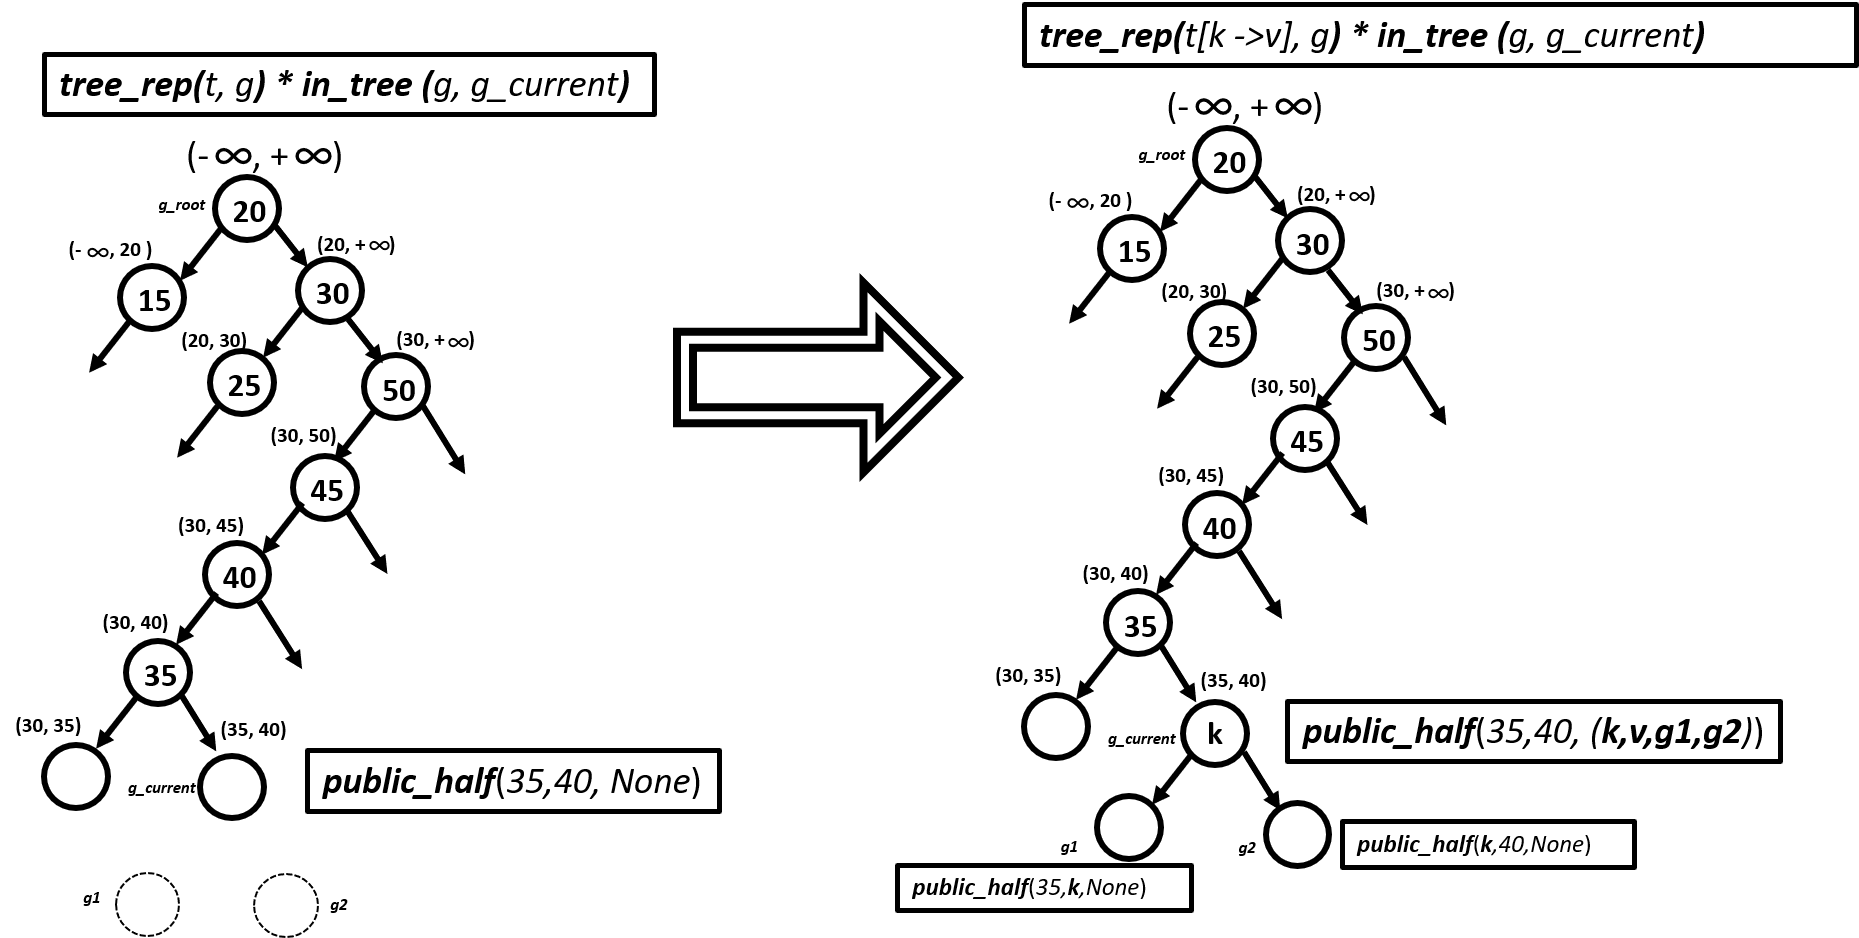
\includegraphics[width=150mm,scale=0.5]{../FIG/extract_insert.png}
\caption{A visual depiction of the change in global state of BST during $\mathsf{insert(k,v)}$ operation }
\label{extract_insert}
\end{figure}
\begin{figure}[htb]
\centering
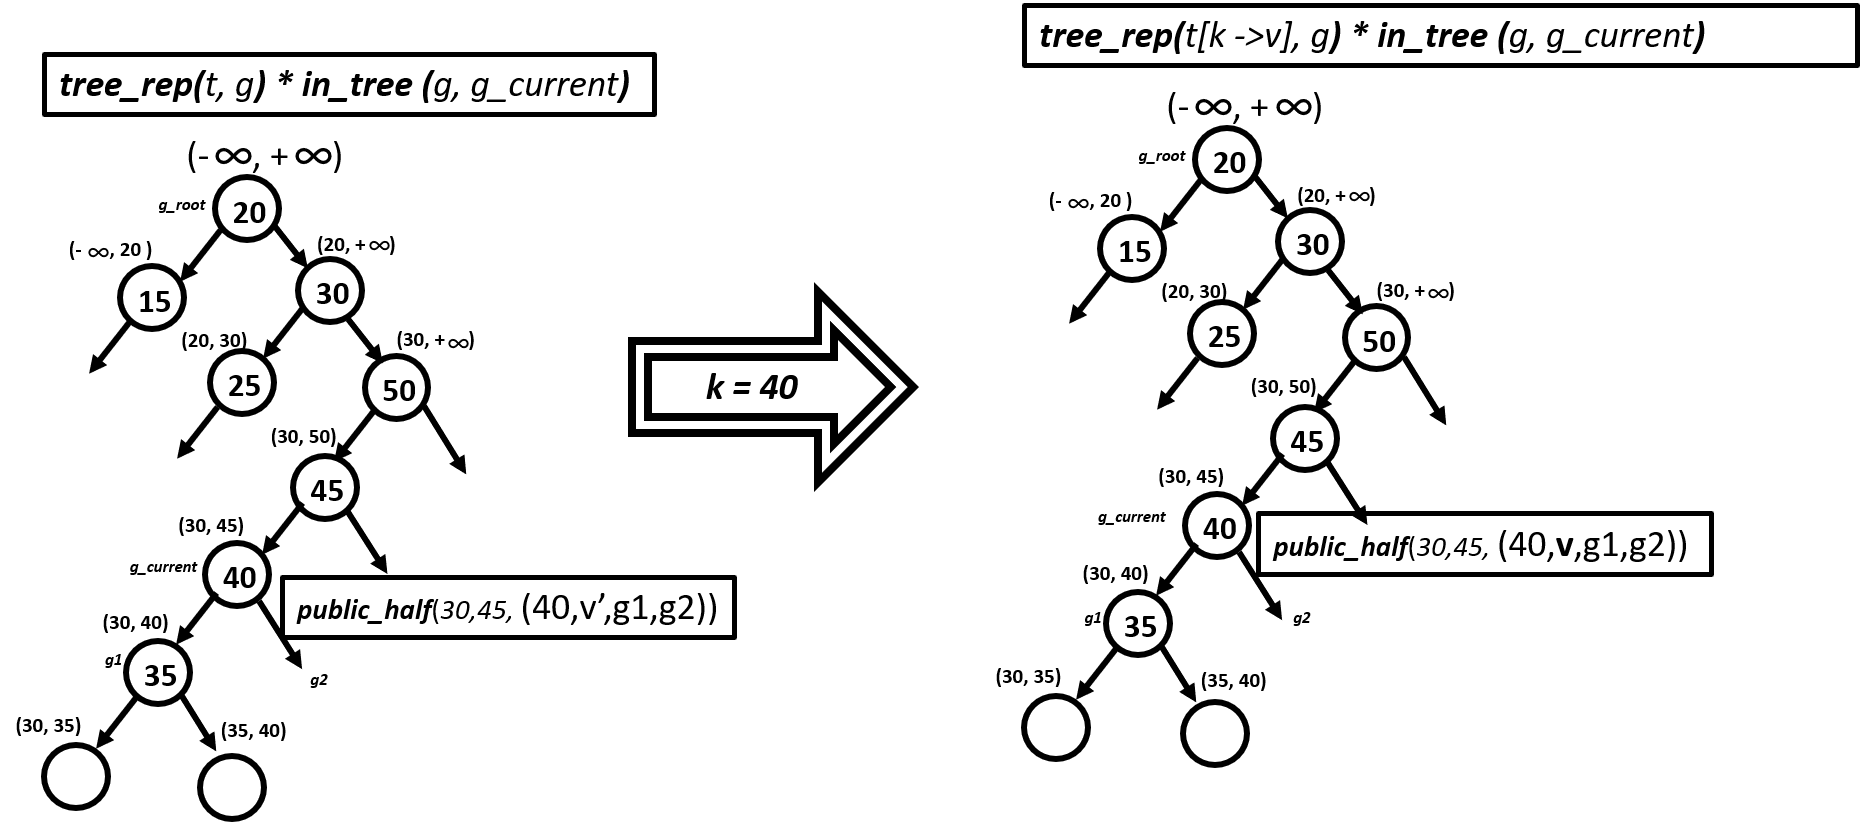
\includegraphics[width=150mm,scale=0.5]{../FIG/extract_insert_2.png}
\caption{A visual depiction of the change in global state of BST during $\mathsf{insert(k,v)}$ operation, where key $k$ already exists in the tree $t$ }
\label{extract_insert2}
\end{figure}

\begin{forest}
for tree={
    grow=south,
    circle, draw, minimum size=3ex, inner sep=1pt,
    s sep=3mm
        }
    [, phantom, for children={fit=band}, s sep+=20mm,
         before drawing tree={%
          tikz+={%
            \node (a) [inner sep=0pt, fit=(!1) (!1L) (!1F)] {};
            \node (b) [inner sep=0pt, fit=(!l) (!lL) (!lF)] {};
            \node [anchor=center] at ($(a.east)!1/2!(b.west)$) {$\longrightarrow\quad$};
          },
        },
        [ 20, tikz={\node[right=0pt of .north east, scale=0.75]  {$(-\infty,\infty)$};}
            [15, tikz={\node[left=0pt of .north west, scale=0.75]  {$(-\infty,20)$};}]
            [30, tikz={\node[right=0pt of .north east, scale=0.75]  {$(20,\infty)$};}
                [25, tikz={\node[left=0pt of .north west, scale=0.75]  {$(20,30)$};}]
                [50, tikz={\node[right=0pt of .north east, scale=0.75]  {$(30,\infty)$};}
                    [45, tikz={\node[left=0pt of .north west, scale=0.75]  {$(30,50)$};}
                        [40, tikz={\node[left=0pt of .north west, scale=0.75]  {$(30,45)$};}
                            [35, tikz={\node[left=0pt of .north west, scale=0.75]  {$(30,40)$};}
                                [, tikz={\node[left=0pt of .north west, scale=0.75]  {$(30,35)$};}]
                                [, tikz={\node[right=0pt of .north east, scale=0.75]  {$(35,40)$}; \node[left=0pt of .west, scale=0.35] {$\mathrm{g\_current}$};}
                                ]
                            ]
                            [$g_2$, draw=none]
                        ]
                        [,no edge, draw=none]
                    ]
                    [,no edge, draw=none]
                ]
            ]
        ]
        [ 20, tikz={\node[right=0pt of .north east, scale=0.75]  {$(-\infty,\infty)$};}
            [15, tikz={\node[left=0pt of .north west, scale=0.75]  {$(-\infty,20)$};}]
            [30, tikz={\node[right=0pt of .north east, scale=0.75]  {$(20,\infty)$};}
                [25, tikz={\node[left=0pt of .north west, scale=0.75]  {$(20,30)$};}]
                [50, tikz={\node[right=0pt of .north east, scale=0.75]  {$(30,\infty)$};}
                    [45, tikz={\node[left=0pt of .north west, scale=0.75]  {$(30,50)$};}
                        [40, tikz={\node[left=0pt of .north west, scale=0.75]  {$(30,45)$};}
                            [35, tikz={\node[left=0pt of .north west, scale=0.75]  {$(30,40)$};}
                                [, tikz={\node[left=0pt of .north west, scale=0.75]  {$(30,35)$};}]
                                [, tikz={\node[right=0pt of .north east, scale=0.75]  {$(35,40)$}; \node[left=0pt of .west, scale=0.35] {$\mathrm{g\_current}$};}
                                ]
                            ]
                            [$g_2$, draw=none]
                        ]
                        [,no edge, draw=none]
                    ]
                    [,no edge, draw=none]
                ]
            ]
        ]
    ]
\end{forest}

\paragraph{Changing the Global State} describe ``extract lemmas'' here---how much detail?

\subsubsection{Lookup}

The code for the $\mathsf{lookup}$ method is shown in Figure
\ref{lookupproof}. It takes the location of the root pointer and a key
as the arguments. A thread spans the tree to find a given key using
hand-over-hand locking mechanism. Once a thread finds the key in the
tree, it gets the value associated with that key, releases the current
node's lock, and returns the value.
The atomic specification for $\mathsf{lookup}$ is
$$\forall t.\ \langle \nodeboxrep\ p\ |\ \treerep\ t\rangle\ \texttt{lookup}(p, k)\ \langle v.\ \nodeboxrep\ p\ |\ \treerep\ t \land \mathrm{lookup}\ t\ k = v\rangle$$
The \texttt{lookup} function should atomically look up the value of the key $k$ in the tree at $p$.

As before, the key to the verification is the invariant for the main loop:
$$\begin{array}{l} \mathsf{lookup\_inv}(b, x, \mathit{g\_root}, \mathit{range},\mathit{info}) \triangleq\ \exists\ \mathit{lock},\ \mathit{g\_current},\ \mathit{np},\ (x\in \mathit{range})\ \land \ \ghost{\mathsf{my\_half}(\mathit{range},\mathit{info})}{\mathit{g\_current}}\\ *\ R\ np\ * \mathsf{lock\_inv}(\mathit{lock},\mathit{lsh2},R')\ *\ \nodeboxrep(b,\mathit{g\_root})\ *\ \mathsf{atomic\_shift} (P_p,E_i,E_o,Q_p,Q) \end{array}$$
where $P_p$ and $Q_p$ are $\treerep(g\_root, t)$ and $(v =
M[k])\ \wedge\ \treerep(g\_root, t)$ respectively. The proof steps for
the $\texttt{lookup}$ verification are similar to the steps
used in $\texttt{insert}$ verification, with a few differences which we
discuss below.

Figure \ref{lookupproof} shows the $\mathsf{lookup}$ function
with separation logic annotations. The proof starts with
$\nodeboxrep$ and $\mathsf{atomic\_shift}$ assertions as the
precondition and follows the same approach as the $\mathsf{insert}$
proof for the verification of loop body. Once we find the target key
(the last $\mathsf{else}$ clause in the code), we need
to confirm that the value present in the tree corresponds with the value we would find if we looked up the key in the current abstract state. We accomplish this by opening the global
invariant encoded in the $\mathsf{atomic\_shift}$, and proving that
lookup satisfies the public postcondition $\mathsf{Q\_p}$ with the help
of the $\mathsf{sync\_commit\_same}$ lemma described in section
\ref{atomicity}. This is the linearization point of the
$\mathsf{lookup}$ operation and must be done before releasing the
current node's lock. When we move into the left or right sub-tree,
we need to establish $\mathsf{lookup\_inv}$ at the end of the $\mathsf{if}$
or $\mathsf{else\ if}$ clause. Here, we need to show that the key we
are searching for is still in the range of our new node, so we use
$\mathsf{sync\_rollback}$ to extract the bound of the left/right
node encoded as the ghost state in the public precondition
($\treerep(M, g, g\_root)$).

A critical difference from $\texttt{insert}$ is that the
$\texttt{lookup}$ method does not change the shape of the tree. With the
help of $\texttt{sync\_commit\_same}$, we need no longer the
heavyweight $\emph{extract}$ lemma but instead a simpler
$\emph{ramif}$ lemma to locate the current node in the global
invariants:
\begin{verbatim}
Lemma ghost_tree_rep_public_half_ramif: forall tg g_root r_root g_in,
Ensembles.In (find_ghost_set tg g_root) g_in -> ghost_tree_rep tg g_root r_root |-- 
EX r: node_info, !! (range_info_in_tree r r_root tg) && (public_half g_in r * 
(public_half g_in r -* ghost_tree_rep tg g_root r_root)).
\end{verbatim}

\begin{figure}[htp]
\begin{subfigure}[t]{1\textwidth}
 $$\left\{\begin{array}{l} \nodeboxrep(b,g\_root)\ *\ \mathsf{atomic\_shift}(P_p,E_i,E_o,Q_p,Q)\end{array}\right\}$$
\begin{lstlisting}[language = C,  numbers = none]
void *lookup (treebox t, int x) {
  struct tree *p; void *v;  struct tree_t *tgt;
  tgt = *t;  void *l = tgt->lock;
  acquire(l);  p = tgt->t;
 \end{lstlisting}  
 $$\left\{\begin{array}{l} \ghost{\mathsf{my\_half}((-\infty,+\infty),info)}{g\_root}\ *\ R\ b\ *\ \mathsf{lock\_inv}(l,lsh2,R')\ *\ \\
 \nodeboxrep(b,g\_root)\ *\ \mathsf{atomic\_shift}(P_p,E_i,E_o,Q_p,Q)\end{array}\right\} \Rrightarrow \left\{\begin{array}{l} lookup\_inv \end{array}\right\}$$ 
  \begin{lstlisting}[language = C, numbers = none]
    while (p!=NULL) {
       \end{lstlisting}   
   $$\left\{\begin{array}{l} lookup\_inv \end{array}\right\} \triangleq \left\{\begin{array}{l}(x\in range)\land \ghost{\mathsf{my\_half}(range,info)}{g\_current}*\ R\ np\ *\\\mathsf{lock\_inv}(lock,lsh2,R')\ *\ \nodeboxrep(b,g\_root)\ *\ \mathsf{atomic\_shift}(P_p,E_i,E_o,Q_p,Q)\end{array}\right\}$$
      \begin{lstlisting}[language = C,  numbers = none]
    if (x<y){
      tgt=p->left;
      ....
    }else if (y<x){
      tgt=p->right;
     ....
    }else {
    v = p->value;
           \end{lstlisting} 
  $$\left\{\begin{array}{l} \ghost{\mathsf{my\_half}(range,info)}{g\_current}*\ R\ np\ *\mathsf{lock\_inv}(lock,lsh2,R')\ *\ \\\nodeboxrep(b,g\_root)\ *\ \mathsf{atomic\_shift}(P_p,E_i,E_o,Q_p,Q)\end{array}\right\} \Rrightarrow{\textbf{sync\_commit\_same}}$$
$$\left\{\begin{array}{l} \ghost{\mathsf{my\_half}(range,info)}{g\_current}*\ R\ np\ *\mathsf{lock\_inv}(lock,lsh2,R')\ *\ \nodeboxrep(b,g\_root)\ *\ Q\end{array}\right\}$$
        \begin{lstlisting}[language = C,  numbers = none]
      release2(l);
         \end{lstlisting}
       $$\left\{\begin{array}{l} \nodeboxrep(b,g\_root)\ *\ Q\end{array}\right\}$$
         \begin{lstlisting}[language = C, numbers = none]
       return v;} }
  release2(l);  return NULL;  }
 \end{lstlisting} 
\end{subfigure}
\caption{The $\texttt{lookup}$ function annotated with separation logic specification}
\label{lookupproof}
\end{figure} 

\subsection{Delete}

The code for the delete method is shown in ??. It takes the location of the root pointer
and a key as the arguments. A thread traverses the tree using hand-over-hand locking,
until the thread finds the key to be deleted. To remove the key, the tree is changed 
through an operation called pushdown left such that the node to be deleted points to an empty leaf
right child. To achieve that, the thread sets the right child's left child as the 
new right child of the to-be-deleted node and moves the right child's right child as 
the new parent of the to-be-deleted node. This operation is repeated until the right
child of the to-be-deleted node is an empty leaf node. Then, the thread will delete
the node and set the delete node's parent pointer to the left child of the deleted node.

The atomic specification for delete method can be written as follows:
$$\forall t.\ \langle \nodeboxrep(p,g,g\_root)\ |\ \treerep(t,g)\rangle $$ 
$$\texttt{delete}(p,k)$$
$$\langle \nodeboxrep(p,g,g\_root)\ |\ \treerep(\texttt{delete}(t, k),g)\rangle $$

The delete method is unique compared to insert and lookup because the pushdown left 
operation can change the \textit{public} half range of more than one nodes. In addition,
the pushdown left operation is one of the main reasons why the ghost tree of the binary
search tree is not just a ``copy" of the pure tree: the functional model of pushdown\_left
is unable to account for the change of deleted node's parent's pointer from pointing
at the deleted node the to the deleted node's right child.



\usetikzlibrary{positioning}

\forestset{
   lab/.style={
        label={[anchor=west, scale=0.75] north east:#1},
    },
}
\begin{forest}
for tree={
    grow=south,
    circle, draw, minimum size=3ex, inner sep=1pt,
    s sep=3mm
        }
    % my label/.style={
        % label={[anchor=south west] north east:#1},
    % },
    [, phantom, for children={fit=band}, s sep+=20mm,
         before drawing tree={%
          tikz+={%
            \node (a) [inner sep=0pt, fit=(!1) (!1L) (!1F)] {};
            \node (b) [inner sep=0pt, fit=(!l) (!lL) (!lF)] {};
            \node [anchor=center] at ($(a.east)!1/2!(b.west)$) {$\longrightarrow\quad$};
          },
        },
        [ 30, tikz={\node[right=0pt of .north east, scale=0.75]  {$(-\infty,\infty)$};}
            [25, tikz={\node[left=0pt of .north west, scale=0.75]  {$(-\infty,30)$};}]
            [75, tikz={\node[right=0pt of .north east, scale=0.75]  {$(30,\infty)$};}
                [40, tikz={\node[left=0pt of .north west, scale=0.75]  {$(30,75)$};}
                    [35, tikz={\node[left=0pt of .north west, scale=0.75]  {$(30,40)$};}]
                    [55, tikz={\node[right=0pt of .north east, scale=0.75]  {$(40,75)$};}
                        [50, tikz={\node[left=0pt of .north west, scale=0.75]  {$(40,55)$};}]
                        [60, tikz={\node[right=0pt of .north east, scale=0.75]  {$(55,75)$};}]
                    ]
                ]
                [80, tikz={\node[right=0pt of .north east, scale=0.75]  {$(75,\infty)$};}]
            ]
        ]
        [ 30, tikz={\node[right=0pt of .north east, scale=0.75]  {$(-\infty,\infty)$};}
            [25, tikz={\node[left=0pt of .north west, scale=0.75]  {$(-\infty,30)$};}]
            [75, tikz={\node[right=0pt of .north east, scale=0.75]  {$(30,\infty)$};}
                [55, tikz={\node[left=0pt of .north west, scale=0.75]  {$(30,75)$};}
                    [40, tikz={\node[left=0pt of .north west, scale=0.75]  {$(30,55)$};}
                        [35, tikz={\node[left=0pt of .north west, scale=0.75]  {$(40,35)$};}]
                        [50, tikz={\node[right=0pt of .north east, scale=0.75]  {$(40,55)$};}]
                    ]
                    [60, tikz={\node[right=0pt of .north east, scale=0.75]  {$(55,75)$};}]
                ]
                [80, tikz={\node[right=0pt of .north east, scale=0.75]  {$(75,\infty)$};}]
            ]
        ]
        [ 30, tikz={\node[right=0pt of .north east, scale=0.75]  {$(-\infty,\infty)$};}
            [25, tikz={\node[left=0pt of .north west, scale=0.75]  {$(-\infty,30)$};}]
            [75, tikz={\node[right=0pt of .north east, scale=0.75]  {$(30,\infty)$};}
                [55, tikz={\node[left=0pt of .north west, scale=0.75]  {$(30,75)$};}
                    [50, tikz={\node[left=0pt of .north west, scale=0.75]  {$(30,55)$};}
                        [40, tikz={\node[left=0pt of .north west, scale=0.75]  {$(30,50)$};}
                            [35, tikz={\node[left=0pt of .north west, scale=0.75]  {$(30,35)$};}]
                            [,no edge, draw=none]
                        ]
                        [,no edge, draw=none]
                    ]
                    [60, tikz={\node[right=0pt of .north east, scale=0.75]  {$(55,75)$};}]
                ]
                [80, tikz={\node[right=0pt of .north east, scale=0.75]  {$(75,\infty)$};}]
            ]
        ]
        [ 30, tikz={\node[right=0pt of .north east, scale=0.75]  {$(-\infty,\infty)$};}
            [25, tikz={\node[left=0pt of .north west, scale=0.75]  {$(-\infty,30)$};}]
            [75, tikz={\node[right=0pt of .north east, scale=0.75]  {$(30,\infty)$};}
                [55, tikz={\node[left=0pt of .north west, scale=0.75]  {$(30,75)$};}
                    [50, tikz={\node[left=0pt of .north west, scale=0.75]  {$(30,55)$};}
                        [35, tikz={\node[left=0pt of .north west, scale=0.75]  {$(30,35)$};}]
                        [,no edge, draw=none]
                    ]
                    [60, tikz={\node[right=0pt of .north east, scale=0.75]  {$(55,75)$};}]
                ]
                [80, tikz={\node[right=0pt of .north east, scale=0.75]  {$(75,\infty)$};}]
            ]
        ]
    ]
\end{forest}

\subsubsection{delete}

Similar with insert, delete starts by acquiring the root node lock, so that the thread
can access the information inside the lock invariant of the root node. Then, we prove
the while loop by showing that the precondition satisfies delete\_inv and the 
loop body preserves the loop invariant. The first two cases are similar to insert and
lookup in which the thread finds the target node, traversing by hand-over-hand locking.
Once the target node is located, the thread will call pushdown\_left and return after.
Using the specification of pushdown\_left, we show that the post-condition of 
pushdown\_left implies the loop invariant. Note that before going into pushdown\_left,
the thread is holding the lock to the target node and will return to the delete
method without holding any.

\subsubsection{pushdown\_left}

The proof to pushdown\_left is the key step of proving the delete method. 
First, we show that the precondition of pushdown\_left satisfies the precondition
of the loop invariant, which includes the assertion that the thread is holding the 
lock to the deleted node (i.e. the information inside the lock invariant is accessible)
and an atomic\_shift. Then, the thread accesses that information to acquire a second 
lock to the right child of the deleted node. Due to the hand-over-hand locking 
mechanism this will not cause a deadlock since the thread has already acquired the 
lock to the deleted node. Next, we prove that the action of deleting the node,
with sync\_commit by opening the global invariant and removing the relevant 
ghost names (the target node and its right sentinel node), satisfies the loop
invariant and the postcondition of pushdown\_left.

The second part of pushdown\_left is proving that the turn\_left operation satisfies
the loop invariant. Using a variant of the sync\_rollback rule, we show that the 
turn\_left operation preserves the BST, apart from changes in the ranges of two nodes,
the target node and its right child, and information about the nodes in those two nodes.
To satisfy the structure of the ranges, we only need to prove that the new range for
the target node is encompasses the old range of both nodes. This will imply that
the range of the target node's old parent includes the target node's right child 
new range as the right child becomes the new parent (and the old parent points to 
the right child).

One key step of the proof is proving that two ghost trees are equivalent if the union
of its ghost nodes are equal and the ghost tree is sorted. This allows the global invariant
to be preserved during the turn\_left operation in which no nodes were actually changed
except for the structure of the tree.


\ignore{\section{Lock-Free BST}
We want to prove that a lock-free BST implementation satisfies the same specification as our hand-over-hand implementation. Unfortunately, provably-correct deletion in a lock-free setting is a research topic in itself (cite?), so we begin with a lock-free BST that only supports insert and lookup. Once again, we want to prove
\begin{mathpar}
\forall t.\ \langle \nodeboxrep\ p\ |\ \treerep\ t\rangle\ \texttt{insert}(p, k, v)\ \langle \nodeboxrep\ p\ |\ \treerep\ (\mathrm{insert}\ t\ k\ v)\rangle

\forall t.\ \langle \nodeboxrep\ p\ |\ \treerep\ t\rangle\ \texttt{lookup}(p, k)\ \langle v.\ \nodeboxrep\ p\ |\ \treerep\ t \land \mathrm{lookup}\ t\ k = v\rangle
\end{mathpar}
though the precise definitions of $\nodeboxrep$ and $\treerep$ will differ. %something about how the fact that the specs are the same really comes across to a client
}

\section{Using the Specifications}
client and client proofs

\section{Related Work}
\label{related}
Gotsman et al.~\cite{gotsman}, in the same paper in which they introduced invariant-style lock specs, also verified a linked list with hand-over-hand locking, which became a common example for CSLs that handled fine-grained locking. Among the most recent of these is the work of Patel et al.~\cite{templates}, who used atomic lock specs to prove correctness of the same data structure. This work updates the work of Gotsman et al. with modern specifications, and directly compares the results to those of Patel et al. 

%Our work is based on the concurrent separation logic of VST in the style of Iris \cite{higherorderghoststate} and the logical atomicity from TaDA logic  \cite{tada}. The notion of the \emph{lower} and \emph{upper} bound is taken from the flow interface paper \cite{krishna2017flow}. Our main technical contributions are the verification of two different implementation of binary search tree (using fine-grained locking and lock-free technique) with respect to the same abstract specification, and first c-level mechanized verification of concurrent search-based data structure (i.e. BST). Most of the other concurrent separation logic (CSL)-based verification works are on toy languages, while VST lets us use the same logic on real C programs.  VeriFast~\cite{verifast-conc} also operates on C code, albeit without a full formal semantics of C.

%Xiong et al. \cite{Xiong2017Abstract} have demonstrated the verification of ConcurrentSkipListMap from java.util.concurrent library using the recent advances in fine-grained concurrency reasoning. Their work is mainly based on the abstract atomicity from TaDA logic, and give two modular specifications for concurrent maps: one specification focus on the entire map structure which is suitable for verifying implementation, and another specification focus on the key-value pairs which appropriate for verifying clients. We use the same idea of atomicity (though implemented in Iris) in our work. 

%TaDA-live: proves atomicity specs of some lock-based data structures incidentally, no mechanization
%search structure templates: lock coupling data structures with atomic specs specifically, really the toy language is the only disadvantage, unclear whether we'd rather replicate them in whole or in part

\section{Conclusion}
\label{conclusion}
While TaDA-style atomic specs for locks have been widely adopted%?
, the implications of the switch away from invariant-based specs had not been thoroughly examined. We have now demonstrated that invariant-based specs can still be used to prove logically atomic specs for larger data structures (even for fine-grained implementations) and that this requires significantly more complex proofs than using atomic lock specs (especially for fine-grained implementations). The old style of lock spec may still be used in systems like VST, where switching would invalidate existing automation or soundness proofs, and in these systems the two-level proof structure we have outlined can be used to obtain strong correctness properties for fine-grained-locking data structures. In all other settings, however, we should strongly prefer to use atomic specifications for locks to simplify our proofs. Indeed, we intend to investigate shifting the foundations of VST to use atomic operations and derive atomic specs for locks: while updating the soundness proof may be an enormous effort, we believe we have shown it to be worth the trouble in the long run.

\subsubsection{Acknowledgements} This work benefited greatly from correspondence with Ralf Jung, who pointed out the atomic syncer example and explained the finer points of logical atomicity in Iris.

%% Bibliography
\bibliography{../sources}
\end{document}
